%!TEX root = ../thesis.tex
%*******************************************************************************
%****************************** Second Chapter *********************************
%*******************************************************************************

\chapter{Quantifying received dose errors introduced by spatial homogenisation of reinforced concrete shielding}
\label{chap:homogenisation}

\ifpdf
    \graphicspath{{Chapter2/Figs/Raster/}{Chapter2/Figs/PDF/}{Chapter2/Figs/}}
\else
    \graphicspath{{Chapter2/Figs/Vector/}{Chapter2/Figs/}}
\fi


\section{Outline}

%INTRODUCTION
\section{Introduction}
An investigation into the process of spatial homogenisation of radiation transport geometry has been performed for reinforced concrete shielding. Using parameters relevant for the ITER fusion experiment, shielding and activation simulations have quantified the effect of homogenisation. The dose received by a person beyond the shield during plasma operation is underestimated by homogenisation. For walls over a meter in thickness it can be by 20\%. The shut down dose to a worker on the tokamak side of an activated wall \textit{due to the wall} is overestimated by homogenisation, by a factor of up to 60.

In nuclear engineering, quantifying the absorbed dose to radiation sensitive components, or the equivalent dose to personnel usually requires crafting a computer model of the problem, making a series of assumptions and simplifications in the process. For reinforced concrete radiation shields, this often entails either homogenising the reinforcing bar (abrev. rebar) with the concrete, or even neglecting the presence of rebar entirely. However, steel has a high density $\sim7.8g\cdot cm^{-3}$ and a markedly different elemental composition to low density $\sim2.2g\cdot cm^{-3}$ concrete. Steel is an alloy of many different elements but principally high-Z Fe. Whereas concrete largely consists of low-Z elements, O, Si \& H (in descending atomic density order).\par
The process of homogenisation introduces systematic error into the reported solution of any radiation transport problem by moving steel and adjusting the density.

The discrepancy in results between heterogeneous and homogeneous modelling approaches is investigated in this work. Querying the strength of correlation of the discrepancy with a given parameter requires producing radiation transport geometry in pairs, as shown in figure \ref{fig:wall_diagram}. 

\subsection{Radiation shielding}
% 

\subsection{Spatial homogenisation}

\subsection{ITER}

% column span figure
\begin{figure}[H]
  \figuretitle{Homogenising reinforced concrete}
	\includegraphics[width=\textwidth]{wall_diagram}
	\caption{The two modelling approaches considered in this investigation. a) Heterogeneous, where the steel reinforcing bar and stirrups are explicitly modelled. b) Homogeneous, where the mass of rebar is 'smeared' through the concrete. The new homogenised material has a greater density than plain concrete, conserving mass.}
	\label{fig:wall_diagram}
\end{figure}

The heterogeneous wall is constructed of a large concrete block, with two meshes of rebar, one buried below each face. The distance from wall exterior to rebar is known as the cover depth. Connecting the two meshes are a small number ($4m^{-2}$) of narrow gauge stirrup bars.

Material compositions, wall widths, rebar arrangements and steel fractions have been determined from ITER drawings and specifications for concrete walls in the tokamak building. The results should give a good idea of the implications of the homogeneous modelling approximation at ITER. The work was also conducted with a moderated ITER DT fusion neutron source spectrum. As such, this investigation should not only be instructive concerning ITER shielding, but also other DT fusion facilities.

%METHOD
\section{Method}

The principal modelling simplification under investigation is that of spatial homogenisation. As such, for each set of independent and dependent variables, at least two simulations will be performed. One will have a high-fidelity model of the real-world problem geometry with rebar and stirrups faithfully reproduced. The other will smear the rebar across the concrete, homogenising the two materials into one with a density equal to the mass weighted sum of the concrete and steel constituents. \par
The implications of homogenisation prove to be different for on-load and shut-down (activated) dose rates. It is helpful to consider them seperately.

\subsection{Prompt neutron \& gamma radiation}

Determining the dose to personnel beyond a wall requires knowledge of the radiation fluxes there. The on-load gamma flux $\phi_{\gamma}(x,y,z,E,t)$ and neutron flux, $\phi_{n}(x,y,z,E)$, can be computed with Monte Carlo techniques, spawning neutrons from a prerecorded source distribution, $P(x,y,z,E,\Omega)$ at a particular point with a given energy and angle. These particles may propagate through the wall, scattering, being absorbed, exciting nuclei (which later relax through radiative emission) and perhaps leaking out of the back of the shield wall. Tallying this leakage flux of neutrons and photons is the main task of calculating a dose due to radiation.\par
Radiation transport was conducted with MCNP6v1.0. The nuclear data employed was the continuous energy Joint Evaluated Fission and Fusion file 3.2 (JEFF3.2) for neutron transport and MCPLIB84 for photon transport. Input decks for MCNP were produced with a bespoke Python program written by the author, this automated approach allowed for easy parametric study. \par
The MCNP relative error, $R = \frac{\sigma_{s}}{\mu_{s}}$ which is the ratio of sample standard deviation to sample mean was kept to below 0.1 for all energy bins and mesh voxels.

% column span figure
\begin{figure}[H]
  \figuretitle{Neutron source spectrum}
	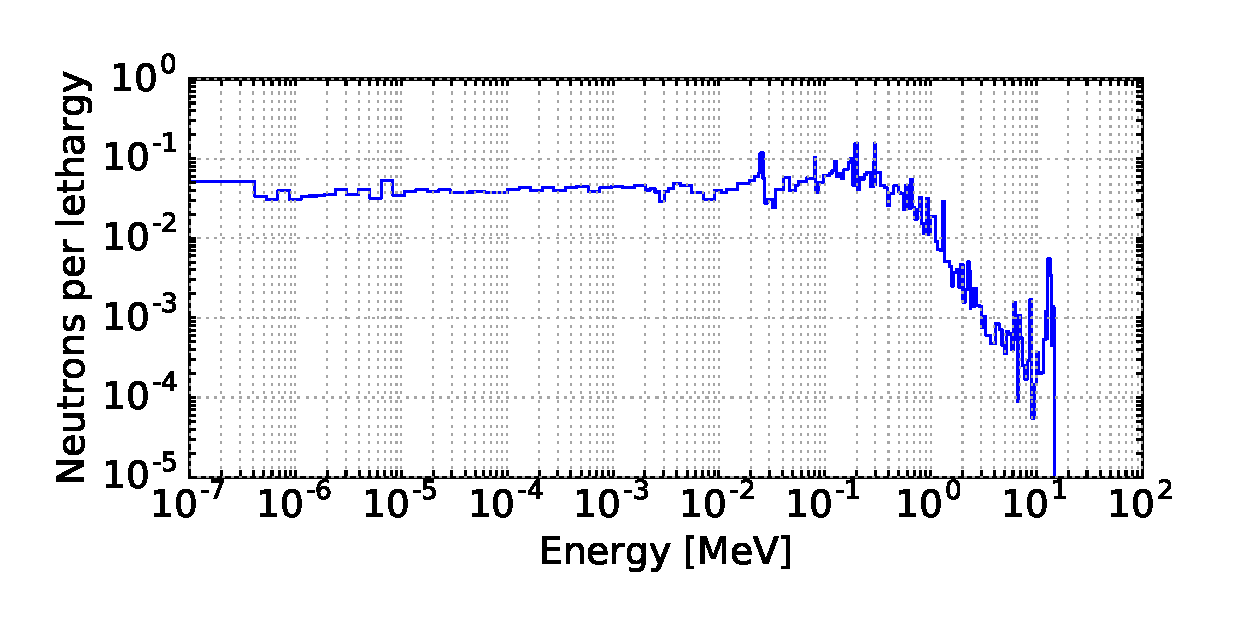
\includegraphics[width=\textwidth]{src_spectra}
	\caption{Neutron spectra for incident radiation. This spectra was recorded in 175 energy groups from the back of the ITER Neutral Beam assembly, immediately inside the bioshield concrete wall.}
	\label{fig:src_spectra}
\end{figure}

The source spectrum plotted as figure \ref{fig:src_spectra} has the recognisable DT peak, but has been significantly thermalised. The apparent absence of a Maxwellian shape around the facility temperature is because of the coarse energy binning used for this tally.

% column span figure
\begin{figure}[H]
  \figuretitle{ICRP74 flux to dose factors}
	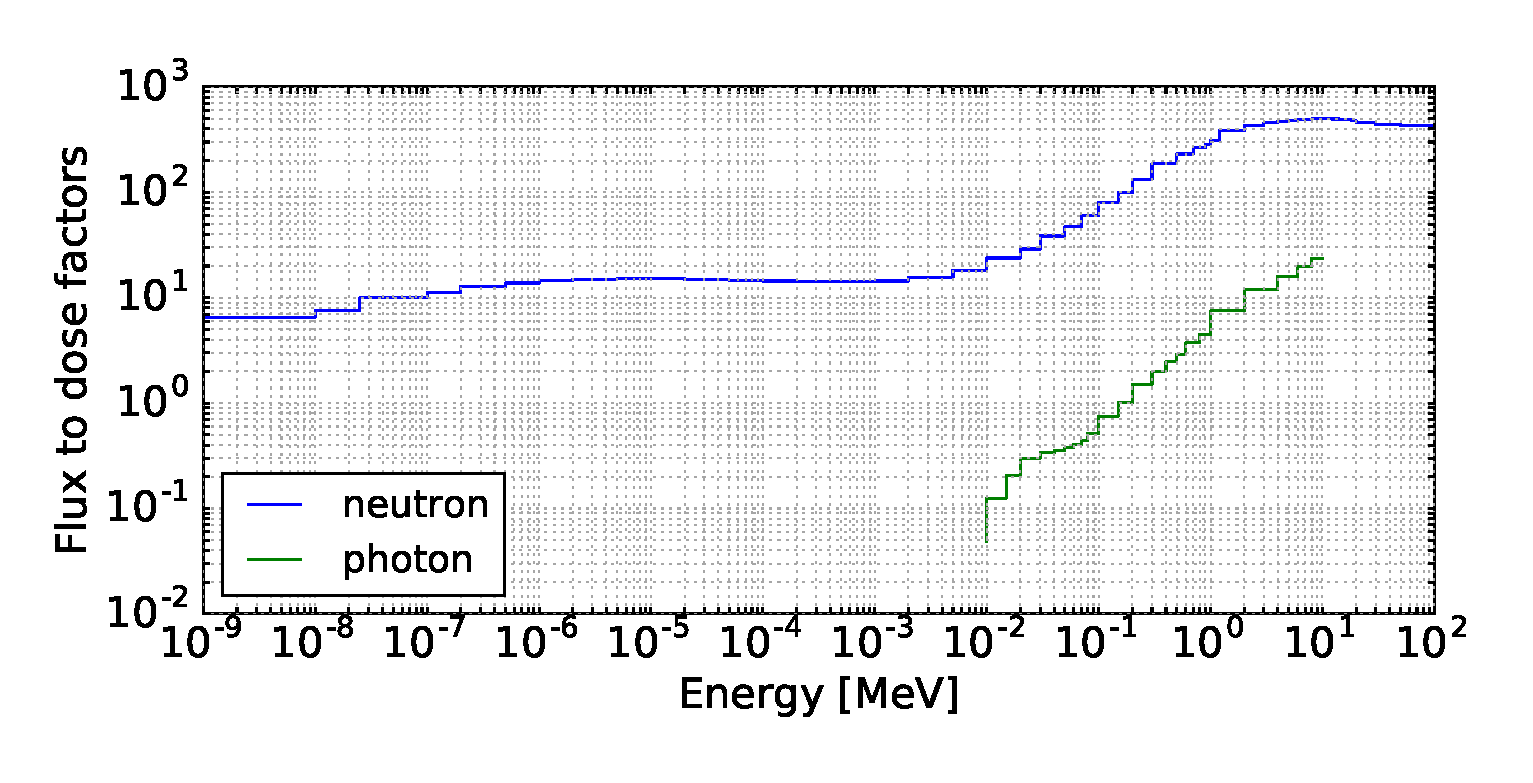
\includegraphics[width=\textwidth]{icrp74}
	\caption{The flux to dose conversion factors for neutron and photon exposure.}
	\label{fig:icrp74}
\end{figure}

The effective dose to humans is a function of the energy and type of radiation. It takes into account the varying susceptibilities of different tissues in the human body. For radiation protection, this is the typical figure quoted when specifying a dose rate. Translation from fluence or flux is by a table similar to that plotted as figure \ref{fig:icrp74}.

%\begin{equation}
%\lambda_{D(e)}=\sqrt{ \frac{ \varepsilon_0 k_B T_{(e)}}{e^2 n_\infty}}
%\end{equation}

\subsection{Delayed gamma radiation}

The calculation of $\phi_{\gamma}(x,y,z,E,t)$ where $t$ is some time after cessation of plasma operation comprises three main steps:
\begin{enumerate}
  \item 1) Neutron transport---as previously, compute the neutron flux during plasma operation, $\phi_{n}(x,y,z,E)$, recording the neutron flux binned by energy over a spatial mesh. 
  \item 2) Activation---determine the appropriate irradiation scenario, then activate and transmutate the materials present in the problem geometry. 
  \item 3) Photon transport---using the distributed decay gamma source produced by step 2), conduct a radiation transport run to determine the photon flux, $\phi_{\gamma}(x,y,z,E,t)$, converting to effective dose as required.
\end{enumerate}

As for before, radiation transport was conducted with MCNP6 v1.0. Activation was conducted with the FISPACT-II code and EAF2010 nuclear data. \par
The irradiation scenario employed for the activation step was ITER's SA-2, which gives a good representation of the ITER experimental programme total fluence and of the final, end-of-life pulses.

%\end{multicols}

%%%%%%%%%%%%%%%%%%%%%%%%%%
% RESULTS AND DISCUSSION %
%%%%%%%%%%%%%%%%%%%%%%%%%%
\section{Results \& discussion}
%\begin{multicols}{2}

\subsection{Transmission of prompt radiation}
\label{subsec:prompt}
The leakage neutron spectra for a thick (2.1m) concrete wall is shown below as figure \ref{fig:trans_neutron_spec}. The flux has been severely reduced by its interaction with the wall, decreasing from the source by an order of magnitude each 20cm traversed.\par
The reduced thermal flux in the homogeneous case is in part because steel is now available for neutron interactions throughout the depth of the wall. Steel has a greater combined capture cross-section than concrete (radiative capture shown in figure \ref{fig:n_rad_capture}), this acts as a neutron sink. 

% column span figure
\begin{figure}[H]
  \figuretitle{Transmitted neutron spectra}
	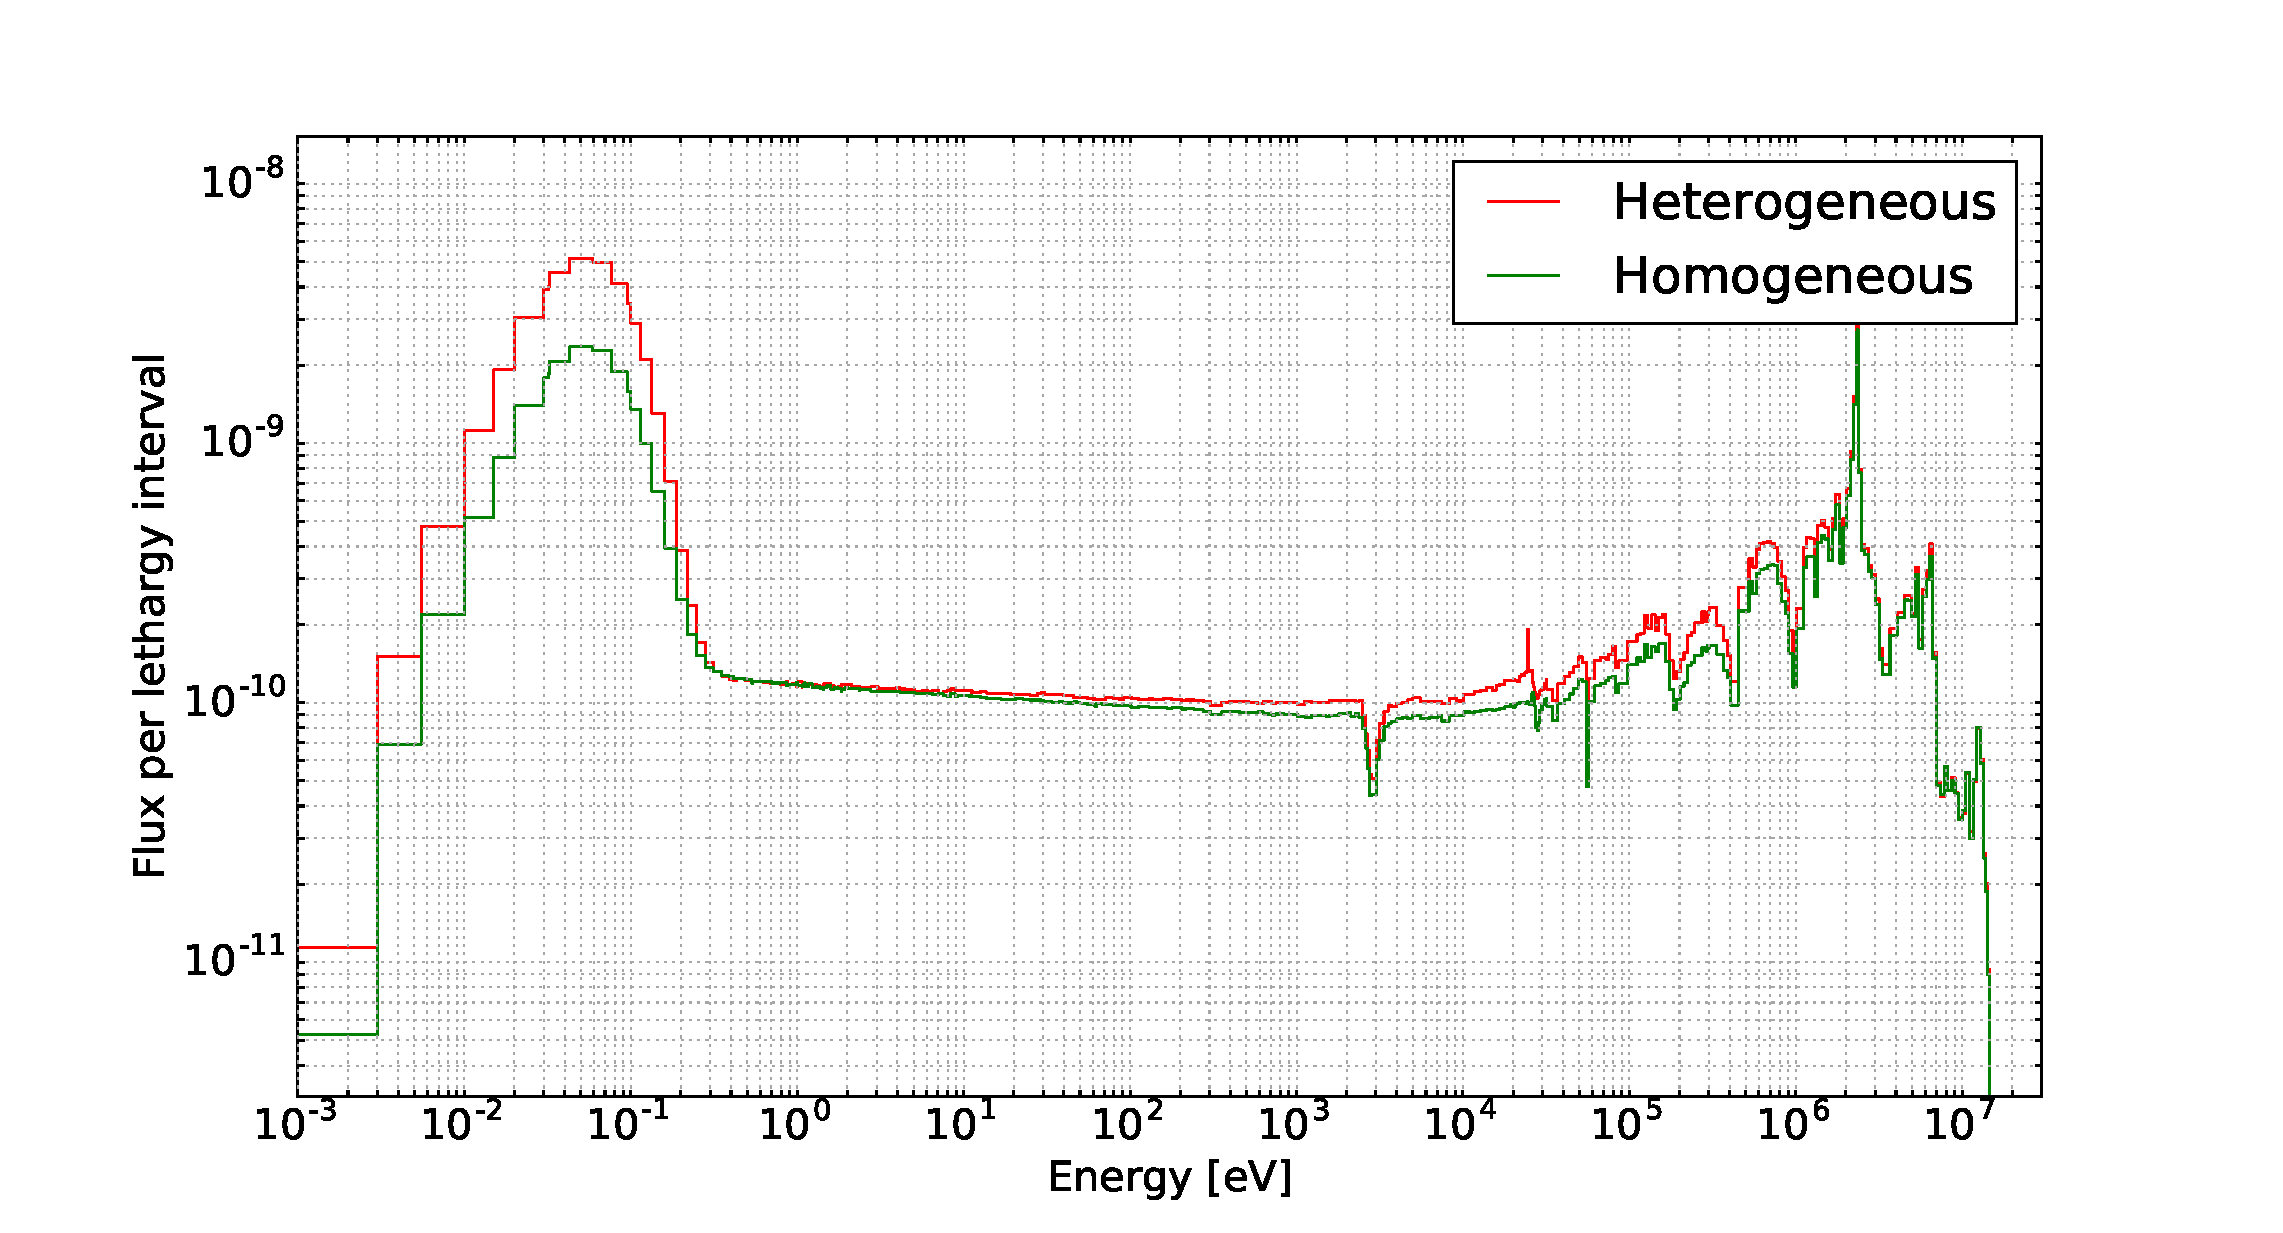
\includegraphics[width=\textwidth]{transmitted_neutron_spectra}
	\caption{The neutron spectra leaving the shield for the heterogeneous and homogeneously modelled cases. Note the substantially reduced thermal flux in the homogeneous simulation. This spectrum has been binned with a finer energy grid than the source, the TRIPOLI 315 group structure.}
	\label{fig:trans_neutron_spec}
\end{figure}

% column span figure
\begin{figure}[H]
  \figuretitle{Radiative capture probability}
  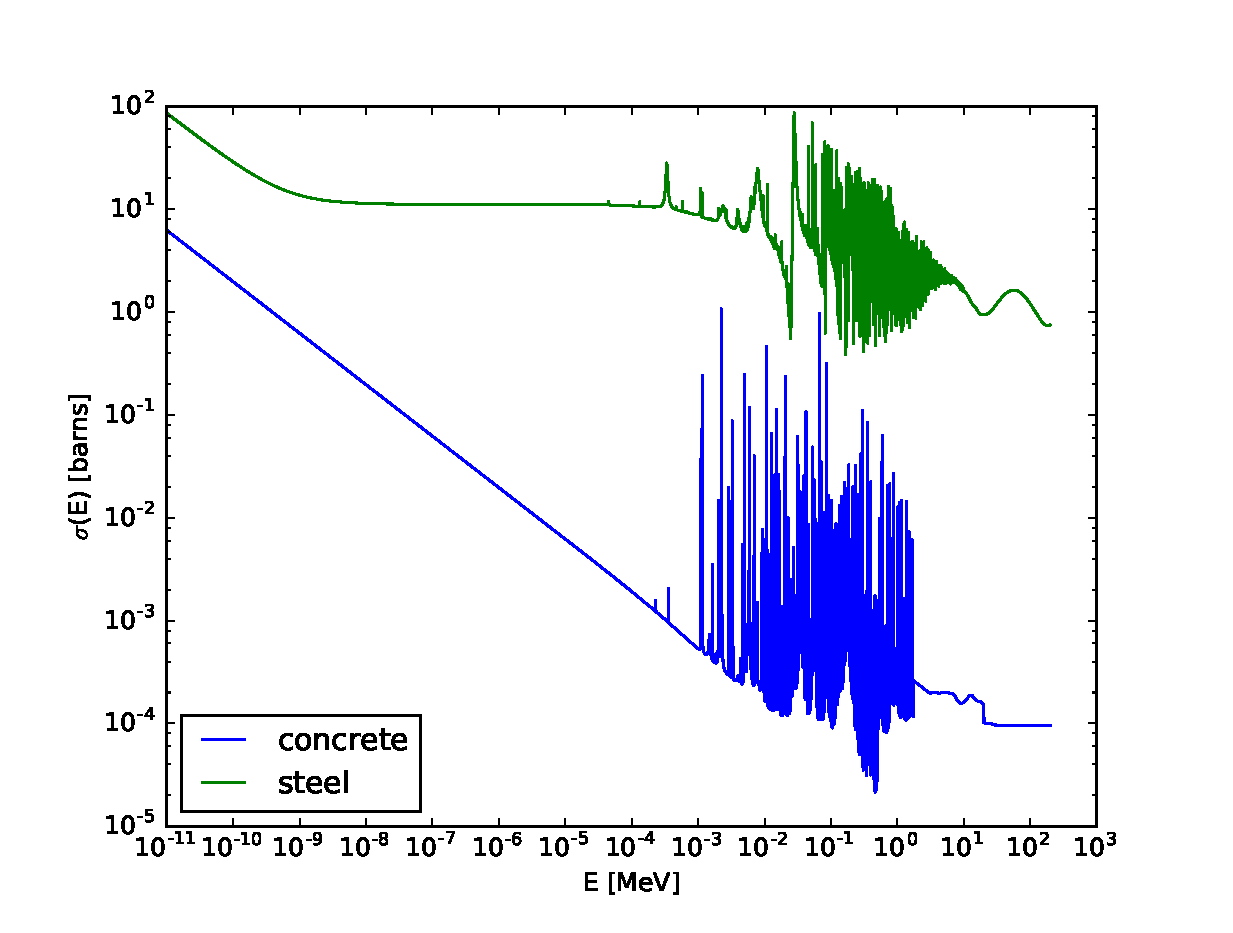
\includegraphics[width=\textwidth]{n_rad_capture}
  \caption{The nuclear properties of steel and concrete are substantially different. Shown here is the cross-section for $(n,\gamma)$ in both materials.}
  \label{fig:n_rad_capture}
\end{figure}

Plotting the ration of the leakage neutron spectra as figure \ref{fig:relative_neutron_spectra} we can see the differences more easily. Thermal flux is underestimated by more than a factor 2. But also, fast flux in the 1keV--1MeV range is underestimated by $\sim1.2$. The fast flux discrepancy is correlated with wall thickness and is negligible for thin (\textless 1m) walls.

% column span figure
\begin{figure}[H]
  \figuretitle{Relative neutron spectra}
	\includegraphics[width=\textwidth]{relative_neutron_spectra}
	\caption{The homogeneous flux increases are readily visible here.}
	\label{fig:relative_neutron_spectra}
\end{figure}

% % column span figure
% \begin{figure}[H]
%   \figuretitle{Contribution to neutron dose}
%   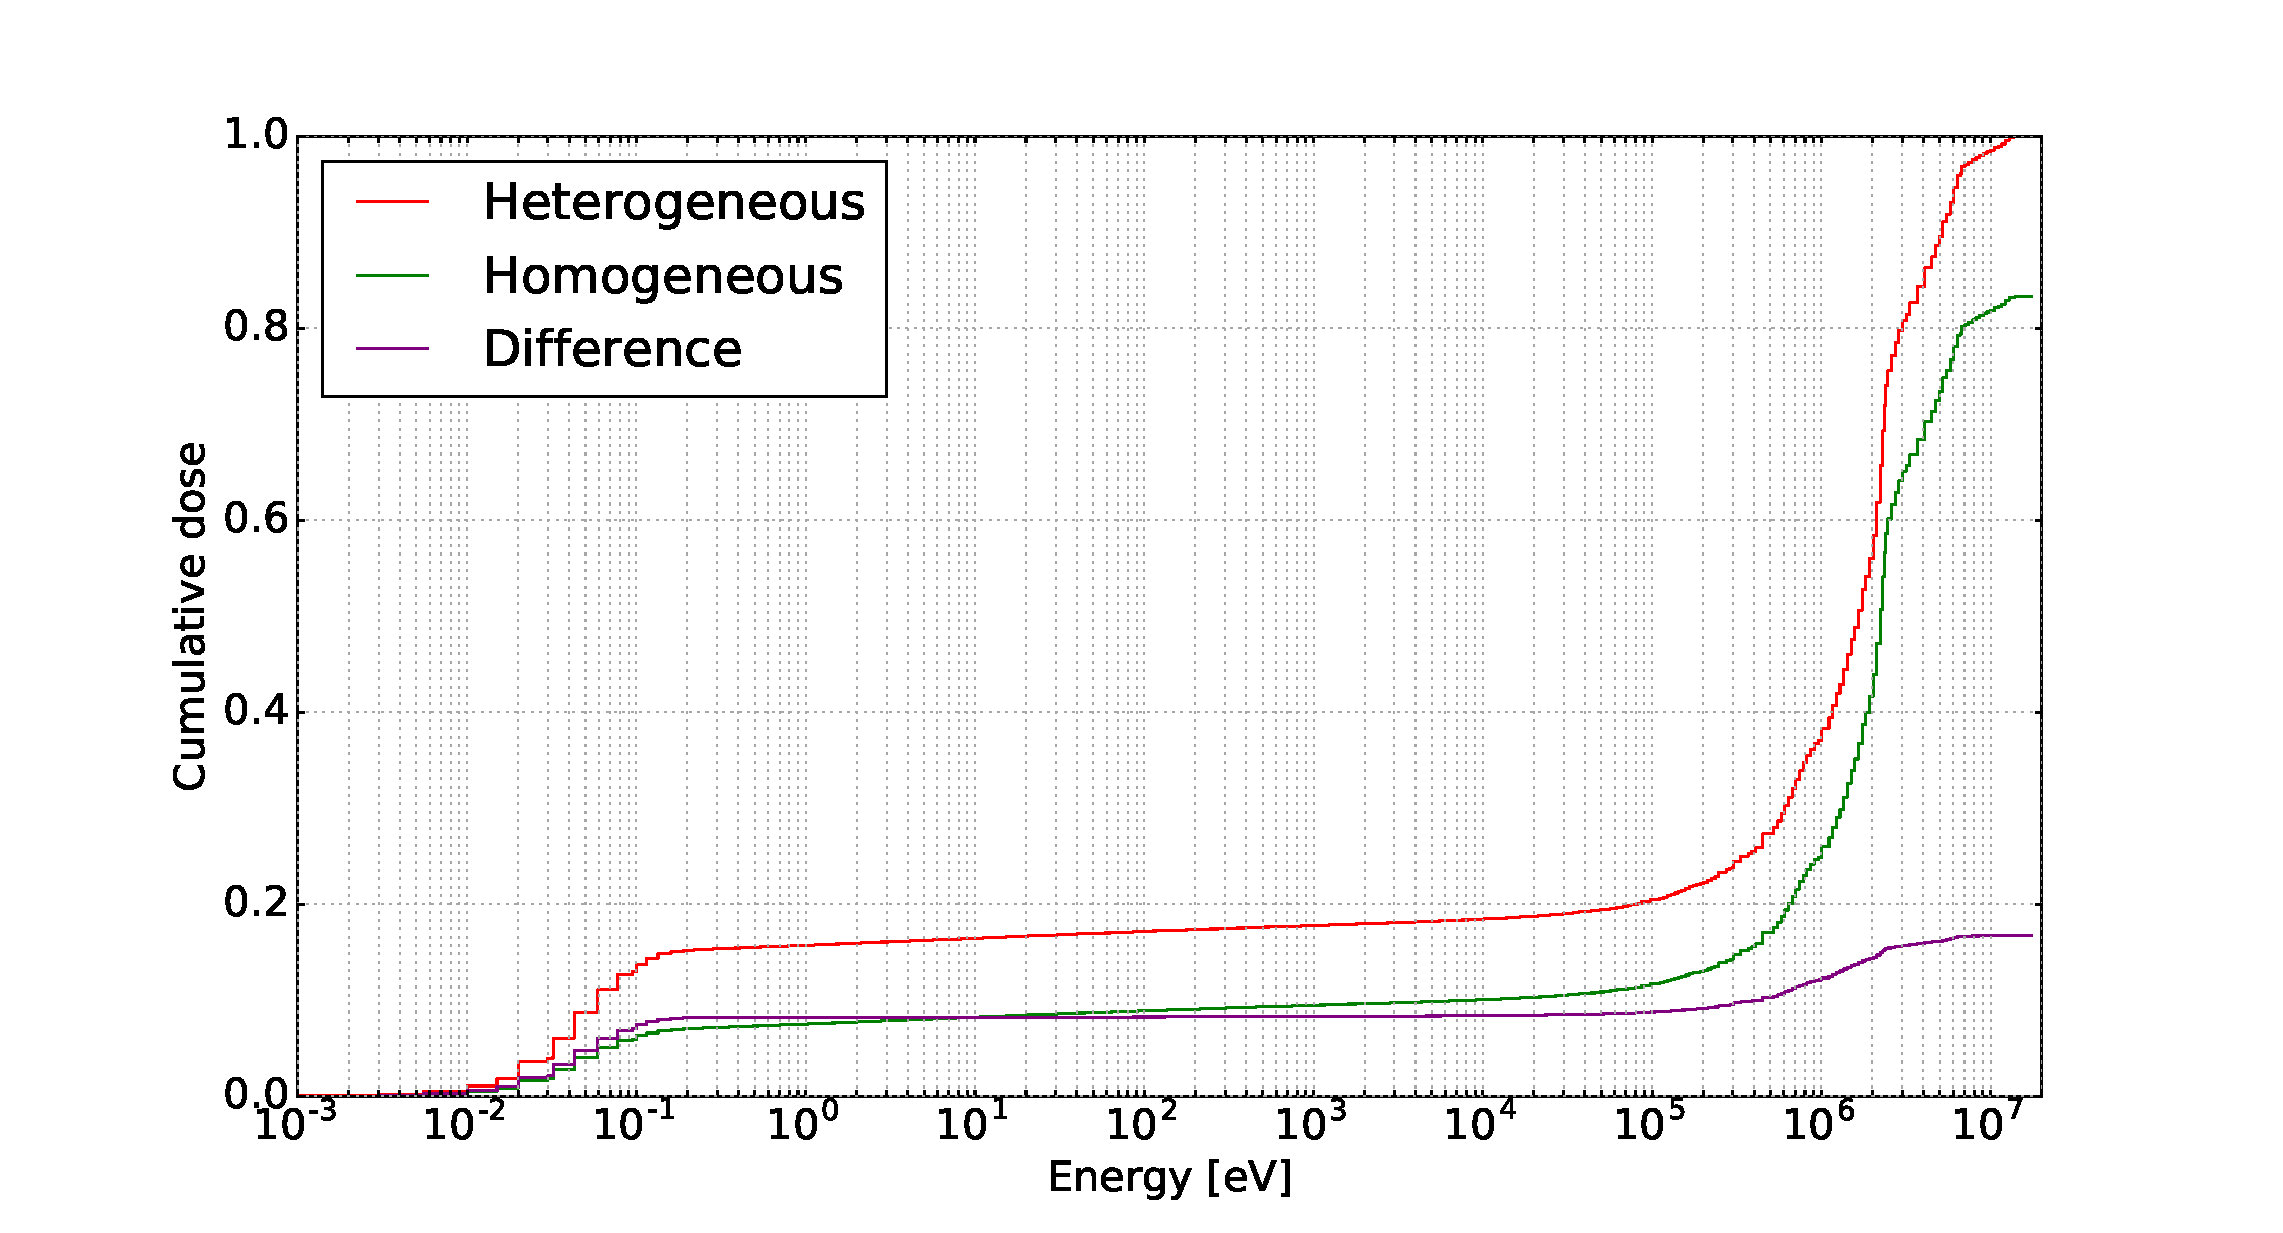
\includegraphics[width=0.5\textwidth]{cumulative_neutron_dose}
%   \caption{Here the dose is cumulatively summed along the energy axis, giving an indication of which energies the dose due to neutrons is from.}
%   \label{fig:cumulative_neutron_dose}
% \end{figure}

Figure \ref{fig:dose_discrepancy} shows how the discrepancy due to the homogeneous approximation varies with wall thickness. It can be seen that the effect is greatest for neutrons. It also plateaus at $\sim 1m$ wall thickness.

% column span figure
\begin{figure}[H]
  \figuretitle{Dose discrepancy due to homogeneity}
	\includegraphics[width=\textwidth]{wall_thickness_dose_discrep}
	\caption{The discrepancy between modelling approaches is a function of the wall thickness for thin walls.}
	\label{fig:dose_discrepancy}
\end{figure}

\subsection{Shut Down Dose Rate}
\label{subsec:sddr}

After operation of a tokamak, repairs and maintenance are often necessary. This section explores the shut-down dose due to be received from the wall itself. It assumes a worker is inside the bioshield at ITER, stood 30cm from the inner surface of an activated wall.\par
Spatial homogenisation acts to overestimate the SDDR beyond 1 day (see figure \ref{fig:sddr}). The homogenised steel in the first few centimeters of the wall is activated by a stronger neutron flux than the physical rebar, located some 5--10cm inside the concrete (the cover depth).

% column span figure
\begin{figure}[H]
  \figuretitle{Shut-down $\phi_{\gamma}$ 30cm from irradiated concrete}
	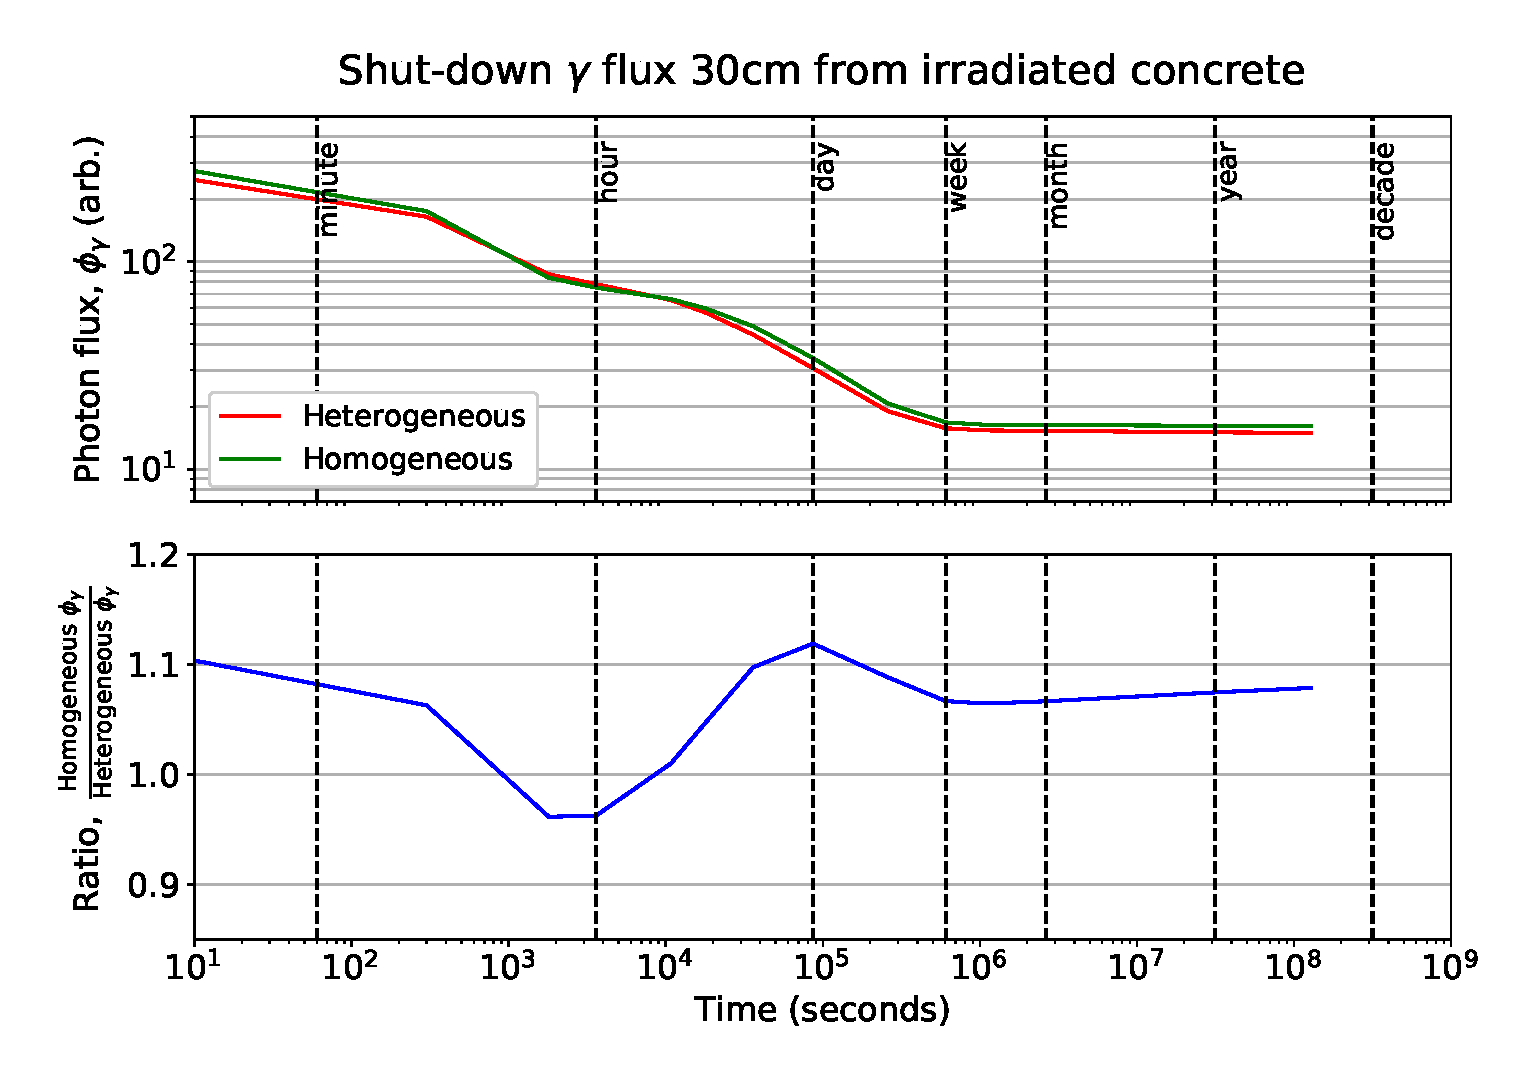
\includegraphics[width=\textwidth]{sddr}
	\caption{The total $\phi_{\gamma}$ as a function of cooling time. The homogeneous simulation gives a significantly increased value at time steps beyond $10^{5}s$ or approximately 1 day.}
	\label{fig:sddr}
\end{figure}

The mean free path of neutrons near the surface is $\sim2cm$ (see figure \ref{fig:mfp}) and as such a typical neutron will undergo several collisions before arriving at the rebar in a heterogeneous simulation. However, in a homogeneous simulation a small amount of steel is present right at the very surface of the concrete, as it is present throughout the simulation. This steel is exposed to an intense neutron flux and is activated accordingly.

% column span figure
\begin{figure}[H]
  \figuretitle{Neutron path length in concrete}
	\includegraphics[width=\textwidth]{mfp}
	\caption{The path lengths of neutrons in pure concrete are shown as a histogram. There is a wide distribution with a mean of approximately 2cm.}
	\label{fig:mfp}
\end{figure}

The plot shown as figure \ref{fig:contact_dose} is produced with data from the activation solver FISPACT-II. Shown are estimates for a contact dose with concrete and steel. As the steel is buried within concrete, the numbers plotted here are not a substitute for transporting decay $\gamma$ photons from their birth to their death. However, they do give a good feel for which nuclides are responsible for the activity of a material at a given time. It is clear that after $^{28}$Al and $^{24}$Na decay in concrete, it has become substantially less active. It is around this time that steel becomes the dominant contributor to dose and the homogeneous modelling approach diverges from heterogeneous.

% column span figure
\begin{figure}[H]
  \figuretitle{Contact dose rate by material}
  \includegraphics[width=\textwidth]{contact_dose_by_mat}
	\caption{This plot shows an estimate for the specific contact dose rate due to steel and concrete irradiated under the ITER SA-2 scenario. Nuclides which contribute a significant fraction of the dose are shown with their abscissa value as their half-life, $t_{\frac{1}{2}}$.}
	\label{fig:contact_dose}
\end{figure}

% % page span figure
% \end{multicols}
% \begin{figure}[H]
%   \begin{center}
%     \includegraphics[width=0.8\textwidth]{contact_dose_by_mat}
%   \end{center}
%   \caption{This plot shows an estimate for the specific contact dose rate due to steel and concrete irradiated under the ITER SA-2 scenario. Nuclides which contribute a significant fraction of the dose are marked.}
%   \label{fig:contact_dose}
% \end{figure}
% \begin{multicols}{2}

\section{Conclusion}
The spatial homogenisation modelling approximation for reinforced concrete underestimates the dose due to neutrons by up to 20\%. The dose due to on-load photons can be underestimated by up to 8\%.\par
The SDDR is instead overestimated by homogenisation, by up to a factor 60 at times beyond a day. 
